% Chapter Template

\chapter{Experiment} % Main chapter title

\label{Chapter4} % Change X to a consecutive number; for referencing this chapter elsewhere, use \ref{ChapterX}

We are trying to estimate the limits of self attribution of a distorted movement. We will do so by estimating the just noticeable difference (JND) in visual stimuli discrepancy. This means estimating the just noticeable \textit{distortion} made to the movement and hence the visual stimuli. The JND is estimated by using the adaptive staircase method introduced by [missing ref].

This method tries to estimate the JND by finding an upper and a lower bound for that value. These are found by changing the intensity of the distortion, based on whether the subject judged the last trial as distorted or not, and the JND is computed as the mean of the last few staircase turns (i.e.\ going from an increasing trend to a decreasing one or vice-versa). The detection judgment is gathered using a Yes/No prompt called the detection question : "Did the movements you saw exactly correspond to the movements you performed?"

\section{Just Noticeable Difference}

The JND will be measured in term of $\gamma$, the gain of the distortion function introduced in Equation \ref{eq:DistortionFunction}. In general, if $\gamma = \SI{-3}{\decibel}$ the subjects are hindered by having to travel two times the distance between the targets, whereas if $\gamma = \SI{3}{\decibel}$ the movement will be amplified and the required motion will be reduced by $50\%$.

Due to the nature of the Egocentric Coordinates and how the distortion is applied (respectively detailed in Chapters \ref{Chapter2} and \ref{Chapter3}), this will not exactly be a metric of the difference in the distance that the subjects have to cover in order to reach the target, such as the metric used by \cite{debarba2017embodiment} [plus other refs]. It however gives a good understanding of the strength and the effect of the applied distortion.

\section{Hypothesis}

The hypothesis we have for the experiment is the following:

\begin{quote}
    \begin{labeling}[:]{H2}
      \item [H1] The absolute value of the JND will be higher when the distortion is positive.
      \item [H2] Do we need more than one hypothesis?
    \end{labeling}
\end{quote}

\section{Equipment and Software}

The HMD used for this experiment is the Oculus Rift in its first consumer version, with a resolution of $1080 \times 1200$ pixels per eye and a refresh rate of \SI{90}{\hertz}.

Some more words on head and body tracking, with references to \cite{molla2013singularity}.

\section{Experiment design}

We manipulate three factors: the sign of the distortion (positive or negative), respectively yielding a helped and hindered movement, the starting value of that distortion (either \num{0} or \SI{9}{\decibel}, and the target sequence (see below). Chapter \ref{Chapter3} gives a complete overview of the concept of distortion and its sign, as well as how it is implemented.

\subsection{Task}

While the whole set of IK goals will be distorted during the experiment, we will be focusing on the dominant hand movement. The task is performed in a seated position in order to avoid any unnecessary movement of the lower limbs, and has the subjects reach three targets. One of them may be in the air in front of them, while the starting and finishing location is the same relative to their skin. The reaching task is performed with the directing hand, and the subjects are instructed to keep their other hand at their side.

\begin{wrapfigure}{r}{.35\textwidth}
    \center{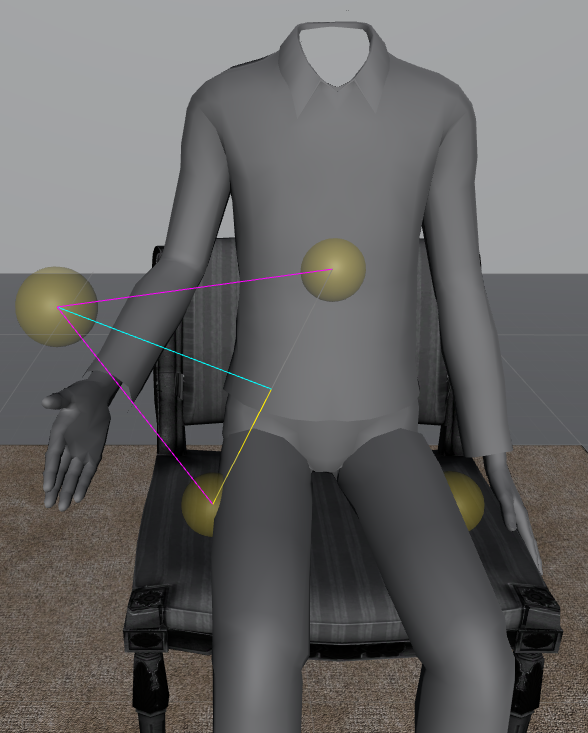
\includegraphics[width=.34\textwidth]
    {Figures/target_placement.png}}
    \caption{An example of target placement with lines showing how its position was reconstructed. The magenta lines are the one of desired length.}\label{fig:targetPlacement}
\end{wrapfigure}

There are four different target orders: \textbf{Chest-Air-Chest}, \textbf{Leg-Air-Leg}, \textbf{Chest-Leg-Chest}, and \textbf{Leg-Chest-Leg}. Both chest and leg targets are located as depicted on Figure \ref{fig:targetPlacement} and are picked according to the subject's handedness: left-handed subjects for instance will have to reach for their left thigh and right shoulder. The first target to be displayed, $T_1$, is always one on the skin and requires the subjects to perform a self-contact in order to activate it. After a random time between \num{200} and \SI{300}{\milli\second}, the target activates. Then the subject moves the hand to the next target, which activates after \SI{100}{\milli\second}. Once this is done the subject goes back to $T_1$, and the detection question is finally asked.

If the sequence requires an intermediary air target, its position is computed such that the subjects have to move a predefined distance $d = 75\%$ of arm length between $T_1$ and $T_{\text{air}}$. Given that a whole sphere of positions is possible, and in order to disambiguate that position, we require that $T_\text{air}$ is also at the same distance $d$ from the third, unused target $T_3$. The air target position therefore is on the intersection between the two spheres of radius $d$ centered on $T_1$ and $T_3$, and we chose the topmost position as a reasonable last disambiguation criterion. Figure \ref{fig:targetPlacement} shows how such position is computed.

One trial---or staircase run---consists of a reaching task, followed by the detection question. Based on the answer to this question, the experiment software modifies the distortion for the next staircase run as follows:
\begin{quote}
    \begin{labeling}{"No" and $\gamma = 0$}
      \item ["Yes"] The discrepancy is increased.
      \item ["No" and $\gamma \neq 0$] The discrepancy is decreased.
      \item ["No" and $\gamma = 0$] The parameter is not changed\footnote{We do not change the distortion in this case because this would invert the sign of the distortion, thus introducing a different distortion.}.
    \end{labeling}
\end{quote}

The amount of each increment or decrement is dynamic: it starts at \num{0.5} and is halved after the first staircase turn. That value is then kept for the rest of that staircase. The staircase is completed either when the subjects change direction 7 times or when they performed 20 trials in that staircase. Figure \ref{fig:trials} shows four instances of ten consecutive trial, depicting the four different initial staircases configuration used for each possible target order.

\begin{figure}[h]
    \center{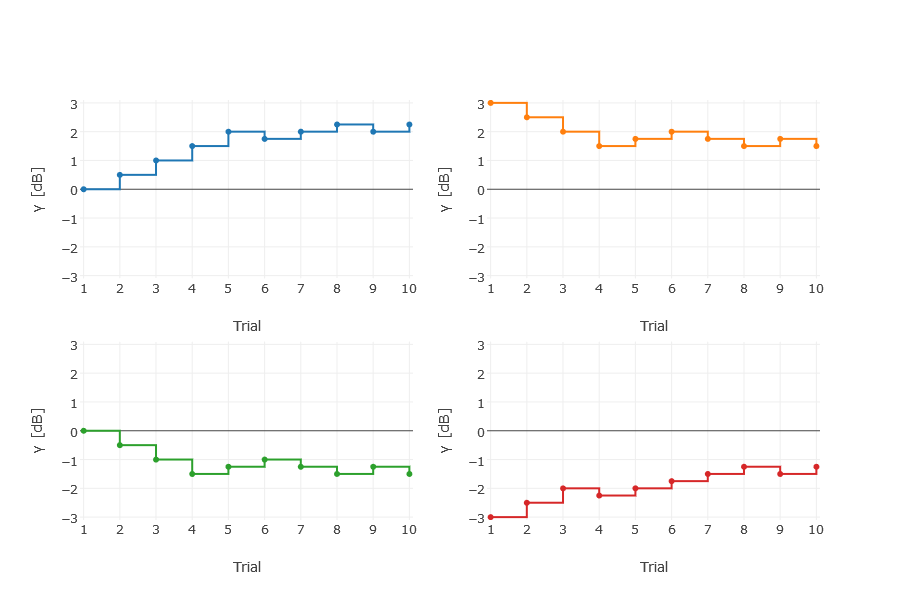
\includegraphics[width=\textwidth]
    {Figures/trials.png}}
    \caption{Four made up partial instances of staircases. Each one features ten trials and four staircases turns, including the one happening in the last trial. The sign of the staircase is the same for each row, while the starting distortion is the same for each column.}\label{fig:trials}
\end{figure}

\subsection{Procedure}

The subjects are welcomed and introduced to the protocol described here, and then introduced to the tracking equipment. A consent form is signed and a characterization form is then filled in by the subjects. The questionnaire features background questions such as age and handedness, but also regarding any previous VR experiment or experience with HMDs. They are then asked to remove their shoes and helped in putting the motion capture suit on. A calibration is then performed as described by \cite{molla2017egocentric} and mentioned in Chapter \ref{Chapter2}.

Before beginning the actual staircase trials, a familiarization phase takes place. The subjects goes through two shortened staircases with constant distortion. The first one has no distortion at all while the second has a big one. The subjects are instructed to always answer ``Yes'' during the first staircase, and ``No'' during the second one, so that they become familiar with the whole procedure.

---at the end of each staircase (max 20 trials) there is a time for the subject to rest, and they are even encouraged to ask for a glass of water if needed. When they are ready to continue, the experimenter presses a button in order to resume the experiment with the next series of trials.

More on the next steps later.

\section{Subjects}

A few physical limitations will be applied to filter the subjects of this experiment. They will be required to be right-handed for ease of software development, and will need to be both smaller than 180cm and have a body mass index between 18 and 27. The latter two criteria are due to our motion capture equipment and especially the suit on which the markers are placed.

We also require that they have a normal or corrected to normal vision, and be fluent in both written and spoken English.
